% National High School Journal of Science Submission
% Compile: pdflatex manuscript.tex (x2), bibtex, pdflatex (x2)

\documentclass[12pt]{article}
\usepackage[margin=1in]{geometry}
\usepackage{setspace}
\doublespacing
\usepackage{times}
\usepackage{amsmath}
\usepackage{booktabs}
\usepackage{graphicx}
\usepackage{caption}
\usepackage{hyperref}
\hypersetup{colorlinks=true,linkcolor=black,citecolor=black,urlcolor=blue}
\usepackage[numbers]{natbib}

\captionsetup{font=small, labelfont=bf}

\begin{document}

% ============================================================
\begin{center}
{\large \textbf{Beyond Accuracy: Investigating Confidence, Calibration,
and Fairness Gaps in a Small Machine Learning Classifier}}

\vspace{0.8em}
{\normalsize Shaurya Gupta}\\
{\small Independent Researcher \quad \href{mailto:shauryagupta042@gmail.com}{shauryagupta042@gmail.com}}

\vspace{0.5em}
{\small \textit{Keywords:} machine learning; calibration; fairness; AUC;
bootstrap uncertainty; small datasets; AI evaluation}
\end{center}
% ============================================================

\begin{abstract}
The most common way to evaluate a machine learning model is to report its AUC
score. I get why---it's clean, it's one number, and it measures something
real. But after spending a few months actually looking at how classifiers get
evaluated in practice, I've started to think AUC consistently hides things
that are worth knowing about.

I trained three classifiers on a small employee attrition dataset (1,470
records) and ran three additional checks beyond AUC: calibration analysis,
bootstrap confidence intervals, and demographic fairness metrics. The AUC
scores all looked reasonable, ranging from 0.759 to 0.798. That's what most
tutorials would call acceptable.

The other results were less reassuring. CatBoost's Expected Calibration Error
was 8.6\%---its probability estimates were off from actual outcome rates by
that much on average. The 95\% bootstrap intervals were 15--16 percentage
points wide, which made me question how much the single reported AUC number
actually means on a dataset this size. And when I split predictions by age
group, the Equalized Odds Difference was 0.258---a 26-point gap that the AUC
never mentioned.

What surprised me most was that all three of these problems appeared at the
same time, in the same model, while the AUC looked fine. That's what
this paper is about.
\end{abstract}

\newpage

% ============================================================
\section{Introduction}
% ============================================================

When someone says an AI system is ``82\% accurate,'' it sounds pretty solid.
More than four out of five predictions correct. But I kept running into a
question I couldn't shake: what does that number actually tell you?

The more I read about machine learning evaluation, the more I realized that
accuracy---and even the more sophisticated version called AUC---leaves out some
things that matter. It doesn't tell you whether the model's confidence
estimates are trustworthy. It doesn't tell you how much the score might vary
if you tested on a different batch of data. It doesn't tell you whether the
errors fall equally on everyone, or whether some groups get worse predictions
than others.

These gaps might not matter much for a model classifying photos of cats versus
dogs. But they matter a lot when the predictions affect real decisions about
people---hiring, lending, medical triage, academic evaluation. In those
contexts, someone is actually acting on the model's output. If the confidence
numbers are off, or if the results are fragile, or if certain groups get
systematically worse predictions, a good AUC score doesn't tell you any of
that.

I wanted to test this directly. I trained three classifiers on a small
organizational dataset and evaluated them with calibration analysis, bootstrap
confidence intervals, and fairness metrics---on top of the standard AUC. The
goal wasn't to build the best-performing model. It was to see whether the AUC
score was telling the full story.

I didn't know going in what I'd find. I expected some calibration issues,
since I'd read that boosted and tree models tend to be overconfident. I didn't
expect the age-based fairness gap to be as large as it came out. And honestly,
the bootstrap results bothered me the most---not because they showed something
broken, but because they made me realize how much uncertainty was hidden behind
a clean-looking single number.

% ============================================================
\section{Background}
% ============================================================

\subsection{What AUC Measures}

AUC stands for area under the ROC (receiver operating characteristic) curve.
The core idea: if you randomly pick one case that's actually positive and one
that's actually negative, AUC tells you how often the model assigns a higher
score to the positive one. An AUC of 0.80 means it gets this right 80\% of
the time. An AUC of 0.50 means it's guessing.

That's a real thing to measure. The problem is that AUC says nothing about
what the actual probability numbers mean. Two models can have the same AUC
while one produces probabilities that closely match actual event rates and the
other is systematically off by a lot. The rankings are identical; the numbers
attached to each prediction can be completely different. If anyone is looking
at those probability numbers to decide how confident to be---which happens a
lot in practice---they're working with two very different tools.

\subsection{Calibration: When Probabilities Should Mean Something}

A well-calibrated model is one where the predicted probability actually
matches the observed frequency. If it says a case has 70\% probability of
the positive outcome, then roughly 70\% of cases with that predicted
probability should actually turn out positive. The weather forecast analogy
is probably the clearest: a meteorologist who says ``70\% chance of rain''
is calibrated if it rains about 70\% of the time when they make that
prediction---not 30\% of the time and not 95\% of the time.

Expected Calibration Error (ECE) is a standard way to measure this
\cite{guo2017}. The idea is to group predictions by confidence level---say,
all predictions between 0.6 and 0.7---and check what fraction of those
actually turned out positive. If the average prediction in that bin is 0.65
but only 0.40 actually turned out positive, that bin contributes a 0.25 gap
to the ECE. Average that across all bins and you get the overall calibration
error. A perfectly calibrated model has ECE of 0.

Tree-based models like random forests and gradient boosting tend to be
overconfident \cite{niculescu2005}. They push probabilities toward 0 and 1
more aggressively than the actual data supports. I was curious whether this
showed up clearly enough to matter, or whether it was just a small
theoretical concern on this dataset.

\subsection{Bootstrap Uncertainty: Is the Score Stable?}

Every test-set evaluation is a single draw from a noisy process. The 294
examples that ended up in my test set are just one possible partition of
the 1,470 total. A different random split would have given a different AUC.
Bootstrap resampling lets you see how sensitive the score actually is: you
resample the data with replacement, re-evaluate many times, and look at how
much the results move. The 95\% confidence interval from that process is more
honest than a single point estimate---it gives you a range of plausible values
instead of pretending the result is more precise than it is.

\subsection{Fairness: Whose Errors?}

Even a classifier with good average accuracy can make worse predictions for
some demographic groups than others. This problem is well-documented---there's
a large literature on sources and types of bias in trained models
\cite{mehrabi2021}. Hardt et al.\ formalized two specific metrics that
are practical to compute \cite{hardt2016}:

\begin{itemize}
  \item \textbf{Demographic Parity Difference (DPD)}: the gap in positive
    prediction rates between two groups.
  \item \textbf{Equalized Odds Difference (EOD)}: the gap in true positive
    \emph{and} false positive rates between groups. A model satisfies
    equalized odds when its error structure is the same regardless of group
    membership.
\end{itemize}

A model can score perfectly on both DPD and EOD and still produce unjust
outcomes if the label itself encodes historical bias---but measuring these
metrics is at least a starting point for understanding whether the classifier
treats groups differently.

% ============================================================
\section{Data and Methods}
% ============================================================

\subsection{Dataset}

I used the IBM HR Analytics Employee Attrition dataset, a synthetic
organizational benchmark publicly available through Kaggle
\cite{ibm2015}. It contains 1,470 employee records described by 35
variables: job characteristics, satisfaction ratings, demographics, and
compensation. The binary outcome is whether the employee left the
organization (attrition); 241 of 1,470 records (16.1\%) are labeled
as attrition events.

The dataset is synthetic---generated by IBM data scientists for
educational purposes, not derived from any real workforce. This matters
for interpreting results: the findings describe model behavior on a
simulated benchmark, not on real employment decisions. That's a meaningful
limitation. It also means the data can be used and shared without privacy
issues, which is why I chose it.

I split the data 80/20 (training: 1,176 records, test: 294) using stratified
sampling to preserve the 16.1\% attrition rate in both sets.

\subsection{Classifiers}

I trained three classifiers:

\begin{enumerate}
  \item \textbf{Logistic Regression (LR)}: a simple linear model that
    produces inherently calibrated probabilities under well-specified
    conditions. Useful as a calibration baseline.
  \item \textbf{Random Forest (RF)}: an ensemble of decision trees. Widely
    used in practice on tabular data \cite{breiman2001}.
  \item \textbf{CatBoost (CB)}: a gradient boosting algorithm with native
    categorical feature handling \cite{prokhorenkova2018}.
\end{enumerate}

I didn't tune hyperparameters. The goal was to see how these classifiers
look under additional evaluation metrics at representative performance
levels, not to squeeze out the best possible AUC.

\subsection{Evaluation}

I evaluated four things:
\begin{enumerate}
  \item \textbf{AUC} on the held-out test set (the standard metric).
  \item \textbf{Expected Calibration Error (ECE)} before and after
    post-hoc calibration correction using isotonic regression.
  \item \textbf{Bootstrap confidence intervals} on AUC: 1,000 resamples,
    reporting the 2.5th and 97.5th percentiles.
  \item \textbf{Fairness metrics} (DPD and EOD) for gender (Male/Female)
    and age group (under~40 / over~40).
\end{enumerate}

All code is publicly available at:
\url{https://github.com/SilverCoin256/accuracy-isnt-enough}

% ============================================================
\section{Results}
% ============================================================

\subsection{AUC: The Baseline Picture}

All three classifiers got AUC scores in the 0.76--0.80 range
(Table~\ref{tab:auc}). Logistic Regression came out on top at 0.798, which
was a little unexpected---simpler models don't always win on tabular data.
These are all meaningfully above the 0.5 random baseline. If this were the
only evaluation, the takeaway would be: all three models work reasonably well,
LR performs best, done.

\begin{table}[htbp]
\centering
\caption{Test-set AUC for each classifier.}
\label{tab:auc}
\begin{tabular}{lc}
\toprule
\textbf{Model} & \textbf{AUC} \\
\midrule
Logistic Regression & 0.798 \\
Random Forest       & 0.759 \\
CatBoost            & 0.762 \\
\bottomrule
\end{tabular}
\end{table}

\subsection{Calibration: The Confidence Scores Were Off}

Table~\ref{tab:ece} shows Expected Calibration Error before and after
applying isotonic regression as a post-hoc calibration correction.

\begin{table}[htbp]
\centering
\caption{Expected Calibration Error (ECE) before and after isotonic
regression calibration correction.}
\label{tab:ece}
\begin{tabular}{lcc}
\toprule
\textbf{Model} & \textbf{ECE (before)} & \textbf{ECE (after)} \\
\midrule
Logistic Regression & 0.047 & 0.058 \\
Random Forest       & 0.032 & 0.036 \\
CatBoost            & 0.086 & 0.066 \\
\bottomrule
\end{tabular}
\end{table}

CatBoost had the worst pre-calibration ECE at 8.6\%, meaning its probability
outputs were off from actual outcome rates by about 9 percentage points on
average. Logistic Regression was at 4.7\%, which is better but still not
nothing. What surprised me about the post-calibration numbers is that LR
actually got slightly \emph{worse} after correction (ECE went from 0.047 to
0.058), while CatBoost improved the most. That's counterintuitive---the model
you'd expect to already be well-calibrated (logistic regression has theoretical
calibration properties under certain conditions) didn't benefit from the
correction step, and the one known for overconfidence did. I'm not sure I have
a clean explanation for it; with only 294 test examples, some of this might
just be noise in the calibration fitting step.

Figure~\ref{fig:calibration} shows a reliability diagram for CatBoost before
correction. The diagonal is perfect calibration. The model's predictions
cluster above the diagonal at the high-confidence end---it's claiming more
certainty than the data supports in exactly the region where decisions are
most likely to get acted on without second-guessing.

\begin{figure}[htbp]
\centering
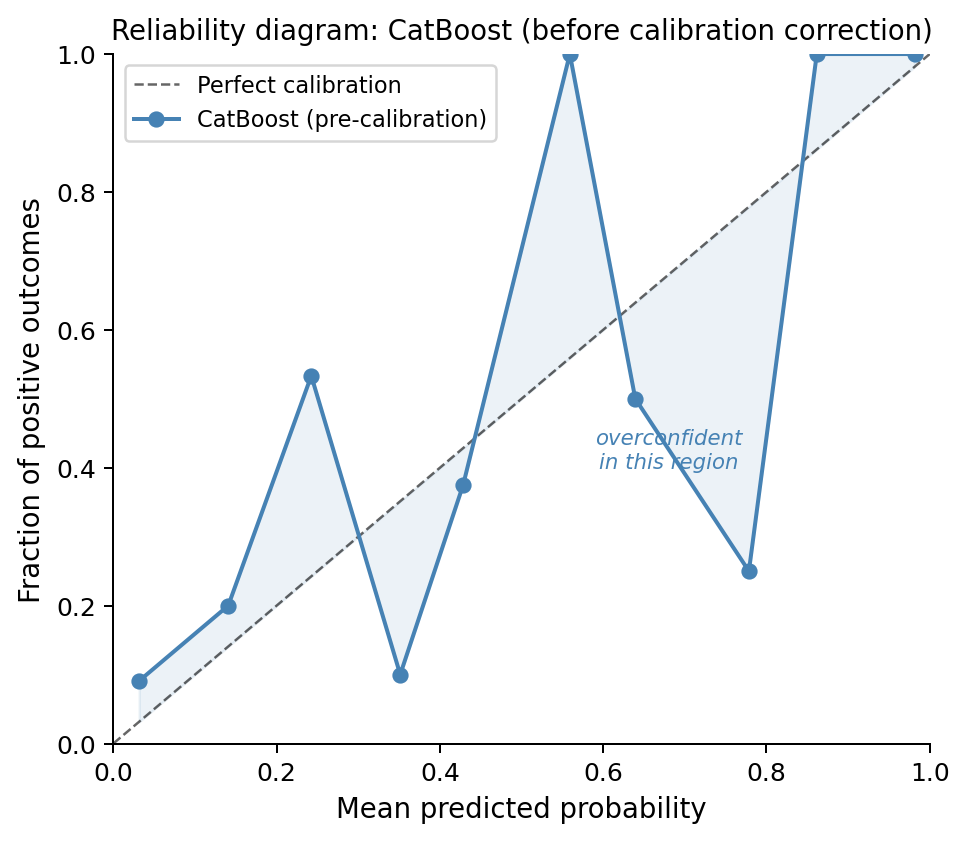
\includegraphics[width=0.7\textwidth]{figures/fig1_reliability_diagram.png}
\caption{Reliability diagram for CatBoost before post-hoc calibration.
  The dashed diagonal represents perfect calibration. The model is
  overconfident, particularly in the high-confidence region (right side
  of the x-axis).}
\label{fig:calibration}
\end{figure}

\subsection{Bootstrap Results: How Stable Are These Scores?}

Table~\ref{tab:bootstrap} shows 95\% bootstrap confidence intervals
on AUC for each model.

\begin{table}[htbp]
\centering
\caption{Bootstrap 95\% confidence intervals on AUC (1,000 resamples).}
\label{tab:bootstrap}
\begin{tabular}{lccc}
\toprule
\textbf{Model} & \textbf{AUC} & \textbf{95\% CI} & \textbf{Width} \\
\midrule
Logistic Regression & 0.798 & [0.716, 0.874] & 0.158 \\
Random Forest       & 0.759 & [0.686, 0.832] & 0.146 \\
CatBoost            & 0.762 & [0.676, 0.838] & 0.162 \\
\bottomrule
\end{tabular}
\end{table}

The intervals are all wide---around 15--16 percentage points for every model.
CatBoost's 95\% interval runs from 0.676 to 0.838. That means if the data
had split differently, the same model and method could have reported an AUC
anywhere in that range. The point estimate of 0.762 is just one draw from
294 test examples out of 1,470 total records.

This bothered me more than the calibration issue. The calibration problem at
least has a known fix---you can apply a correction layer and it usually
helps. The bootstrap result doesn't have a fix; it's just an honest
description of what 1,470 records can and can't tell you. The reported AUC
isn't wrong, exactly. It's just less precise than it looks. On a larger
dataset the confidence intervals would narrow. On this one, they don't, and
presenting just the point estimate without this context seems misleading.

Figure~\ref{fig:bootstrap} shows the bootstrap distribution of CatBoost AUC
scores across all 1,000 resamples.

\begin{figure}[htbp]
\centering
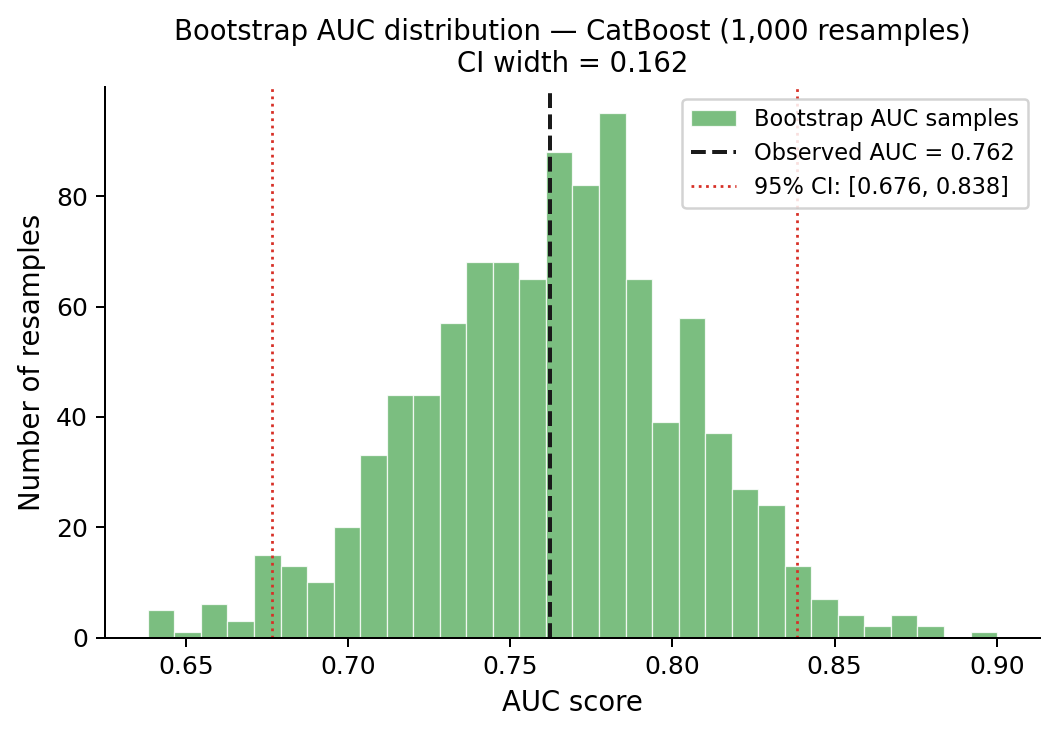
\includegraphics[width=0.72\textwidth]{figures/fig2_bootstrap_distribution.png}
\caption{Bootstrap distribution of CatBoost AUC across 1,000 resamples.
  The vertical dashed line marks the observed test AUC. The shaded region
  shows the 95\% confidence interval. The distribution is fairly spread,
  showing meaningful sensitivity to which samples ended up in each set.}
\label{fig:bootstrap}
\end{figure}

\subsection{Fairness: Age-Based Disparities Were Large}

Table~\ref{tab:fairness} shows demographic parity difference and equalized
odds difference for gender (Male vs.\ Female) and age group (under~40
vs.\ over~40), using CatBoost predictions.

\begin{table}[htbp]
\centering
\caption{Fairness metrics for CatBoost. DPD = Demographic Parity Difference;
  EOD = Equalized Odds Difference. Smaller values are better.}
\label{tab:fairness}
\begin{tabular}{lcc}
\toprule
\textbf{Group} & \textbf{DPD} & \textbf{EOD} \\
\midrule
Gender (Male vs.\ Female) & 0.018 & 0.026 \\
Age (Under~40 vs.\ Over~40)   & 0.062 & 0.258 \\
\bottomrule
\end{tabular}
\end{table}

Gender disparity was small: DPD of 0.018 and EOD of 0.026. The model
predicts attrition for male and female employees at similar rates and
with similar error structures. The age disparity was different. EOD of
0.258 means there was a 26-percentage-point gap in equalized odds between
younger and older employee groups---a substantial difference in how
accurate the model was for each group, despite having the same overall
AUC.

To be clear: this finding has to be interpreted carefully on a synthetic
dataset. The IBM HR data was generated by IBM, not collected from a real
organization, so the age disparity might reflect an artifact of how the
simulation was constructed rather than a pattern that generalizes. But
that's exactly the point: the age-based EOD of 0.258 showed up regardless,
and it's the kind of thing the overall AUC score never hints at.

Figure~\ref{fig:fairness} shows the EOD comparison across groups.

\begin{figure}[htbp]
\centering
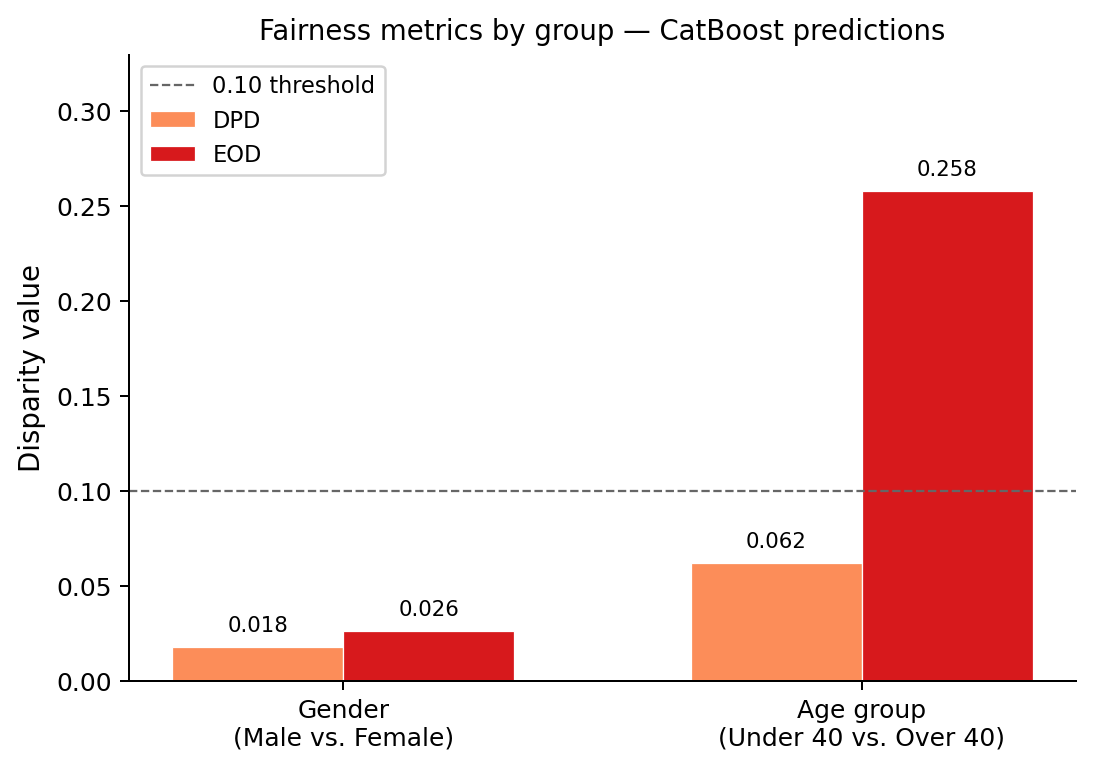
\includegraphics[width=0.65\textwidth]{figures/fig3_fairness_comparison.png}
\caption{Equalized Odds Difference for gender and age group using
  CatBoost predictions. The dotted reference line at 0.10 marks a
  commonly used threshold for acceptable group disparity. The age-group
  EOD of 0.258 substantially exceeds it.}
\label{fig:fairness}
\end{figure}

% ============================================================
\section{Discussion}
% ============================================================

\subsection{What These Results Say Together}

The thing that struck me reviewing these results is that none of the three
problems I found are weird edge cases. Overconfident probabilities,
sensitivity to data splits, uneven errors across demographic groups---these
aren't exotic failure modes that only appear in unusual circumstances. They
appeared together, in the same models, on a standard benchmark dataset that
most ML tutorials would describe as a working example of good performance.

The calibration problem means someone relying on these probability outputs
would be working with numbers that are more confident than they should be.
The bootstrap problem means the AUC headline figure is a less stable estimate
than it looks on a dataset this small. The fairness problem means the model
made noticeably different kinds of errors for different age groups, and
nothing in the AUC score hinted at that.

None of this makes the models useless. But it makes them harder to trust
than a single number suggests---and I think that's worth saying clearly.

\subsection{Why Small Datasets Make This Worse}

Part of what makes these findings concerning is the dataset size. With 1,470
records, the problems I found---uncertain AUC estimates, noisy calibration
correction, unstable fairness metrics across small demographic subgroups---are
partly a function of how little data there is. More records would help with
all of them. Wider bootstrap intervals, noisier calibration fits, less
reliable fairness metrics per subgroup are all normal consequences of small
$n$.

But here's the thing: 1,470 records isn't unusual for real deployment
settings. School districts, small healthcare clinics, local government
agencies, small companies---these are exactly the places where AI tools are
being adopted, and their datasets are often this size or smaller. The
evaluation problems I found here probably aren't edge cases. They're probably
what things look like in practice a lot of the time.

\subsection{Post-Hoc Calibration: Helps, But Not Always}

Post-hoc calibration reduced ECE for CatBoost from 0.086 to 0.066---roughly
a 23\% improvement. Random Forest also improved slightly. But Logistic
Regression actually got marginally worse (0.047 to 0.058). I mentioned this
earlier and I still don't have a clean explanation; my best guess is that with
only about 200 examples in the calibration fitting set, there wasn't enough
data to estimate a reliable correction for LR, which was already better
calibrated to begin with.

The practical point is that calibration correction is useful, especially for
models like CatBoost that are known to be overconfident. But it's not a free
win---it requires setting aside calibration data you might not have to spare,
and the correction itself can be noisy at small sample sizes. I wouldn't treat
it as a guaranteed improvement on datasets smaller than this one.

\subsection{What I'd Do Differently}

A few honest reflections on limitations and what I'd change:

The dataset is synthetic. I chose it because it's clean, reproducible, and
publicly available---but IBM generated it for educational purposes, not from
a real workforce. Some of what I found, especially the age-based fairness
gap, might be an artifact of how the simulation was constructed. I can't
know. The right next step would be running the same evaluation on a real
organizational dataset, with actual demographic variation, to see if the
patterns hold.

I also didn't tune hyperparameters. That was intentional---the goal was to
see how these models perform under default settings, not optimized ones. But
it means the AUC scores are probably not the best each model could do, which
might affect where calibration error ends up.

The one question I'm most curious about: does the age disparity survive
after calibration correction? I noticed the age-group EOD was high for
CatBoost, and CatBoost was also the most miscalibrated model. Those might be
connected. If the calibration fix also reduces the fairness gap, that would
be an interesting result. I didn't check this in the current analysis because
the calibration correction didn't produce uniform improvements across models,
and I wasn't confident the result would be interpretable on this sample size.

% ============================================================
\section{Conclusion}
% ============================================================

I started this project curious about whether AUC was really sufficient for
evaluating classifiers, or whether it was just the metric everyone used
because it was easy and familiar. The answer I found, at least on this
dataset, is that it's insufficient in ways that are pretty easy to demonstrate
with standard tools.

The calibration analysis, bootstrap intervals, and fairness metrics I ran
aren't advanced research methods. They're all available in scikit-learn and
take maybe a few extra hours to implement on top of whatever pipeline already
produces AUC. The information they return is genuinely different from what AUC
tells you.

What I came away from this project thinking is that the gap between a model
that ``achieves 0.80 AUC'' and a model that's actually ready to be trusted in
a real decision-making context is larger than most evaluations acknowledge.
The three models I tested cleared the AUC bar without clearing the
calibration, stability, or fairness bars. Whether that gap matters depends
on context---but I think you have to check before you can know. And right
now, most evaluations don't check.

I don't think this is the final word on anything. It's a small study on a
synthetic benchmark, and I've noted the limitations throughout. There's a
wider argument in the literature that messy evaluation practices in ML lead to
real downstream problems when these systems get deployed \cite{sculley2015},
and I think the results here are at least a small illustration of why. The
core question---what does a performance metric not tell you---is worth
asking earlier and more routinely than it currently is.

% ============================================================
\section*{Data Availability}
% ============================================================

IBM HR Analytics Employee Attrition dataset: publicly available on Kaggle at
\url{https://www.kaggle.com/datasets/pavansubhasht/ibm-hr-analytics-attrition-dataset}

% ============================================================
\section*{Code Availability}
% ============================================================

All analysis code and figure generation scripts are available at:
\url{https://github.com/SilverCoin256/accuracy-isnt-enough}

% ============================================================
\section*{AI Assistance Disclosure}
% ============================================================

Generative AI tools were used for code formatting and citation lookup.
All analysis decisions, interpretations, and manuscript writing
were conducted by the author.

% ============================================================
\begin{thebibliography}{9}

\bibitem{breiman2001}
L.~Breiman, ``Random forests,''
\textit{Machine Learning}, vol.~45, pp.~5--32, 2001.

\bibitem{guo2017}
C.~Guo, G.~Pleiss, Y.~Sun, and K.~Q.~Weinberger,
``On calibration of modern neural networks,''
in \textit{Proc.\ 34th Int.\ Conf.\ Machine Learning (ICML)},
pp.~1321--1330, 2017.

\bibitem{hardt2016}
M.~Hardt, E.~Price, and N.~Srebro,
``Equality of opportunity in supervised learning,''
in \textit{Advances in Neural Information Processing Systems}, vol.~29,
pp.~3323--3331, 2016.

\bibitem{ibm2015}
IBM Data Scientists,
``IBM HR Analytics Employee Attrition \& Performance [Synthetic dataset],''
Kaggle, 2015. [Online]. Available:
\url{https://www.kaggle.com/datasets/pavansubhasht/ibm-hr-analytics-attrition-dataset}

\bibitem{mehrabi2021}
N.~Mehrabi, F.~Morstatter, N.~Saxena, K.~Lerman, and A.~Galstyan,
``A survey on bias and fairness in machine learning,''
\textit{ACM Computing Surveys}, vol.~54, no.~6, Article~115, 2021.

\bibitem{niculescu2005}
A.~Niculescu-Mizil and R.~Caruana,
``Predicting good probabilities with supervised learning,''
in \textit{Proc.\ 22nd Int.\ Conf.\ Machine Learning (ICML)},
pp.~625--632, 2005.

\bibitem{prokhorenkova2018}
L.~Prokhorenkova, G.~Gusev, A.~Vorobev, A.~V.~Dorogush, and A.~Gulin,
``CatBoost: Unbiased boosting with categorical features,''
in \textit{Advances in Neural Information Processing Systems}, vol.~31,
2018.

\bibitem{sculley2015}
D.~Sculley \textit{et al.},
``Hidden technical debt in machine learning systems,''
in \textit{Advances in NIPS}, vol.~28, pp.~2503--2511, 2015.

\end{thebibliography}

\end{document}
